\chapter{Algoritam Sparc}

Cilj ovog projekta bio je implementirati algoritam Sparc \citep{ye2016sparc} koji se koristi u konsenzus fazi preklapanje-razmještanje-konsenzus (engl. Overlap-Layout-Consensus, OLC) pristupa.
Sparc je algoritam za konsenzus fazu OLC pristupa, temeljen na \emph{k-mer/de Bruijn} \citep{hannenhalli1996positional} grafovima.

\section{Ulaz u algoritam}
TODO: seke
Algoritam koristi izlaz iz faze razmještanja OLC pristupa te sva početna očitanja genoma.
Očitanja su mapirana na kontigu iz faze razmještanja i pohranjena u datoteku formata .sam, opisanom u nastavku.

Kako bi uspješno izgradili graf i proveli algoritam, potrebno je znati gdje se pojedina očitanja mapiraju na osnovnu kontigu.
Te informacije dobivano iz .sam datoteke koju smo generirali alatom \emph{GraphMap} \citep{sovic2016fast}.
Nama najvažnije informacije u datoteci jesu:
\begin{description}
  \item [POS] pozicija na osnovnoj kontizi na kojoj počinje mapiranje pojedinog očitanja
  \item [CIGAR] operacije obavljene nad očitanjem kako bi se dobilo mapiranje (dodavanje, brisanje, pomicanje, itd.)
  \item SEQ: očitana sekvenca u prvotnom obliku (bez obavljenih CIGAR operacija)
  \item [QUAL] kvaliteta očitanja (iz .fastq datoteke očitanja)
\end{description}

Važnost navedenih informacija bit će jasnija kasnije.
Za naše potrebe, spremili smo sve važne informacije u zasebnu datoteku koja se sastoji od osnovne kontige (engl. backbone, layout) u prvoj liniji.
U nastavku datoteke su očitanja zapisana kroz tri linije.
Prva linija predstavlja originalno očitanje na koje su primjenjene CIGAR operacije kako bi se dobilo poravnanje s backbone-om.
U drugoj liniji nalazi se kvaliteta očitanja (QUAL), a u trećoj je pozicija na backbone-u na kojoj počinje mapiranje izmjenjene sekvence.

\section{Opis algoritma}
Temeljni dio algoritma je izgradnja grafa $k$-mera. Prvi korak u izgradnji spomenutog grafa jest pretvorba referentong genoma \engl{backbone} u sparse lanac $k$-mera kao što je prikazano u $(a)$ dijelu slike. Gustoću grafa korigiramo hiperparametrom $g$, dok je veličina $k$-mera određena parametrom $k$. U čvorovima lanca nalaze se $k$-meri dok se na vezama nalaze dijelovi genoma koji ih povezuju. 

Uz referentni genom imamo i niz očitanja koja se djelomično ili potpuno mapiraju na taj genom, a opis jednog takvog očitanja vidljiv je u prethodnom odlomku. Koristeći očitanu sekvencu [SEQ] i niz operacija nad tom sekvencom [CIGAR] gradimo mapiranje na referentni genom koje u odnosu na njega može imati neke elemente zamijenjene, obrisane ili dodane. Od tog mapiranja gradimo lanac k-mera sličan lancu referentnog genoma uz dodatak što svaki puta kada novoizgrađeni čvor već postoji u stablu k-mera, prethodni čvor ćemo, uz odgovarajući prijelaz, samo spojiti na njega. Ovaj dio algoritma lijepo je vidljiv u (b) i (c) dijelovima slike 2.1.

Primijetimo sada da je graf k-mera usmjeren i acikličan \engl{DAG - Directed Acyclic Graph}, a skup svih lanaca tog grafa nam predstavlja prostor rješenja. Kako bismo izabrali najizgledniji lanac, uz oznaku prijelaza svake veze pamtit ćemo i neku mjeru izglednosti da je baš ta veza dio optimalnog lanca. Ovu mjeru možemo modelirati na razne načine, a u našoj implementaciji je ona jednaka broju očitanja čiji lanci prolaze tom vezom. Izglednost nekog lanca modelirana je sumom težina svih veza tog lanca. Dakle, problem smo sveli na traženje najduljeg puta u DAG-u. Primijetimo da nam usmjerenost i acikličnost dopuštaju nešto efikasniji pronalazak najduljeg puta u grafu. Naime, svaki DAG ima barem jedan topološki poredak čvorova \engl{Topological sort} pa se problem najdužeg puta svodi na jednostavno dinamičko programiranje. Neka $dist_i$ označava najdulji put nekog lanca koji završava u čvoru koji se u topološkom poretku nalazi na poziciji $i$. Tada vrijedi relacija $dist_i = max\{dist_j + w_{ji}\}$ za svaki čvor koji se u topološkom poretku nalazi na indeksu $j$ i direktno je povezan s čvorom na indeksu $i$. Postojanje topološkog poretka nam garantira da ćemo prije $dist_i$ već imati izračunate sve vrijednosti $dist_j$ pa najdulji put nalazimo u složenosti $O(V+E)$.   

\begin{figure}[htb]
\centering
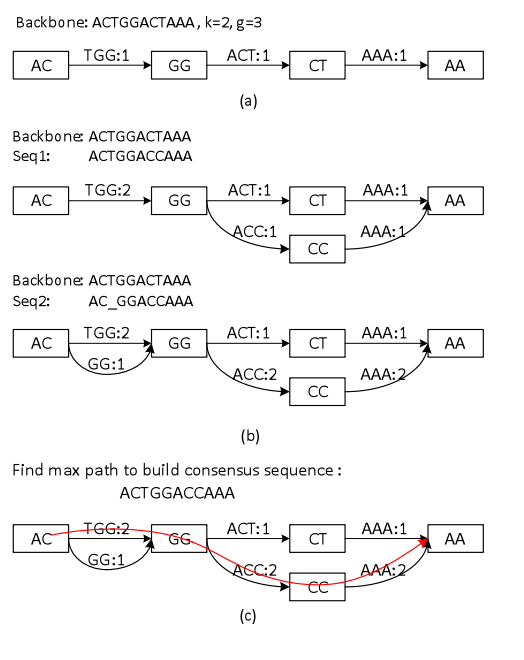
\includegraphics[scale=0.6]{figures/sparc.png}
\caption{Izgradnja grafa.}
\label{fig:sparc}
\end{figure}

